% Options for packages loaded elsewhere
\PassOptionsToPackage{unicode}{hyperref}
\PassOptionsToPackage{hyphens}{url}
\documentclass[
]{article}
\usepackage{xcolor}
\usepackage[margin=24mm]{geometry}
\usepackage{amsmath,amssymb}
\setcounter{secnumdepth}{-\maxdimen} % remove section numbering
\usepackage{iftex}
\ifPDFTeX
  \usepackage[T1]{fontenc}
  \usepackage[utf8]{inputenc}
  \usepackage{textcomp} % provide euro and other symbols
\else % if luatex or xetex
  \usepackage{unicode-math} % this also loads fontspec
  \defaultfontfeatures{Scale=MatchLowercase}
  \defaultfontfeatures[\rmfamily]{Ligatures=TeX,Scale=1}
\fi
\usepackage{lmodern}
\ifPDFTeX\else
  % xetex/luatex font selection
\fi
% Use upquote if available, for straight quotes in verbatim environments
\IfFileExists{upquote.sty}{\usepackage{upquote}}{}
\IfFileExists{microtype.sty}{% use microtype if available
  \usepackage[]{microtype}
  \UseMicrotypeSet[protrusion]{basicmath} % disable protrusion for tt fonts
}{}
\makeatletter
\@ifundefined{KOMAClassName}{% if non-KOMA class
  \IfFileExists{parskip.sty}{%
    \usepackage{parskip}
  }{% else
    \setlength{\parindent}{0pt}
    \setlength{\parskip}{6pt plus 2pt minus 1pt}}
}{% if KOMA class
  \KOMAoptions{parskip=half}}
\makeatother
\usepackage{graphicx}
\makeatletter
\newsavebox\pandoc@box
\newcommand*\pandocbounded[1]{% scales image to fit in text height/width
  \sbox\pandoc@box{#1}%
  \Gscale@div\@tempa{\textheight}{\dimexpr\ht\pandoc@box+\dp\pandoc@box\relax}%
  \Gscale@div\@tempb{\linewidth}{\wd\pandoc@box}%
  \ifdim\@tempb\p@<\@tempa\p@\let\@tempa\@tempb\fi% select the smaller of both
  \ifdim\@tempa\p@<\p@\scalebox{\@tempa}{\usebox\pandoc@box}%
  \else\usebox{\pandoc@box}%
  \fi%
}
% Set default figure placement to htbp
\def\fps@figure{htbp}
\makeatother
\setlength{\emergencystretch}{3em} % prevent overfull lines
\providecommand{\tightlist}{%
  \setlength{\itemsep}{0pt}\setlength{\parskip}{0pt}}
\usepackage{mathrsfs}
\usepackage{mathtools}
\DeclareUnicodeCharacter{2212}{\ensuremath{-}}

\DeclareUnicodeCharacter{2265}{\ensuremath{\ge}}
\DeclareUnicodeCharacter{2264}{\ensuremath{\le}}
\DeclareUnicodeCharacter{2295}{\ensuremath{\oplus}}
\DeclareUnicodeCharacter{2297}{\ensuremath{\otimes}}
\DeclareUnicodeCharacter{2208}{\ensuremath{\in}}
\DeclareUnicodeCharacter{2261}{\ensuremath{\equiv}}
\DeclareUnicodeCharacter{21A6}{\ensuremath{\mapsto}}
\DeclareUnicodeCharacter{2192}{\ensuremath{\to}}
\DeclareUnicodeCharacter{03BA}{\ensuremath{\kappa}}
\DeclareUnicodeCharacter{039B}{\ensuremath{\Lambda}}
\DeclareUnicodeCharacter{03C4}{\ensuremath{\tau}}
\DeclareUnicodeCharacter{03A9}{\ensuremath{\Omega}}
\usepackage{bookmark}
\IfFileExists{xurl.sty}{\usepackage{xurl}}{} % add URL line breaks if available
\urlstyle{same}
\hypersetup{
  hidelinks,
  pdfcreator={LaTeX via pandoc}}

\author{}
\date{}

\begin{document}

{
\setcounter{tocdepth}{3}
\tableofcontents
}
\section{The cross-effect retained by a contractible
complex}\label{the-cross-effect-retained-by-a-contractible-complex}

The nonzero cohomology produced from a split contractible complex is an
explicit cross-effect. This paper computes its maps, group-ring
multiplication, full scalar action and augmentation filtration. It also
computes a nonzero torsion-input example whose entire associated graded
object and augmentation completion vanish, preserving the original
object and the kernel of that completion map.

\subsection{1. The free construction and its
cross-effect}\label{the-free-construction-and-its-cross-effect}

For an abelian group \(V\), write
\(U(V)=\bigoplus_{v\ne0}\mathbb Zr_v\), with \(r_0=0\), and
\(U(f)r_v=r_{f(v)}\). Define \(\epsilon_V:U(V)\to V\) by
\(r_v\mapsto v\), and \(K(V)=\ker\epsilon_V\). The multiplicative monoid
ring \(\Lambda=\mathbb Z[\mathbb Z\setminus\{0\}]\) acts by
\([n]r_v=r_{nv}\). Composition of integer multiplications proves the
scalar action law; every U(f) is \(\Lambda\)-linear.

For abelian groups A,B, let \(i_A,i_B\) and \(p_A,p_B\) be the
inclusions and projections of \(A\oplus B\). Define \[
\operatorname{cr}_2U(A,B)=
\ker\bigl(U(p_A)\oplus U(p_B):U(A\oplus B)\to U(A)\oplus U(B)\bigr).
\tag{X1}
\] \textbf{Theorem X1.} There is a natural direct sum decomposition \[
U(A\oplus B)=U(A)\oplus U(B)\oplus W(A,B),
\qquad W(A,B)\cong U(A)\otimes_{\mathbb Z}U(B),
\tag{X2}
\] whose first two inclusions are \(U(i_A),U(i_B)\), and whose third
inclusion is \[
\kappa(r_a\otimes r_b)
=w_{a,b}:=r_{(a,b)}-r_{(a,0)}-r_{(0,b)}.
\tag{X3}
\] The third summand is exactly (X1). Its projection is \[
\Pi=1-U(i_Ap_A)-U(i_Bp_B).
\tag{X4}
\]

\textbf{Proof.} The original free basis splits into the symbols on the
nonzero A-axis, the nonzero B-axis, and those \(r_{(a,b)}\) with both
a,b nonzero. Replace each symbol in the last family by (X3). This is an
invertible basis change: its inverse writes
\(r_{(a,b)}=w_{a,b}+r_{(a,0)}+r_{(0,b)}\), leaving both axis bases
fixed. The projections kill exactly the third summand and recover the
two axis coordinates, proving every asserted kernel and decomposition.
Their composite idempotents on \(U(A\oplus B)\) are orthogonal, because
\(p_Ai_B=p_Bi_A=0\) and U(0)=0; therefore (X4) is the projection onto
their common kernel. The tensors \(r_a\otimes r_b\), a,b nonzero, form
the free tensor-product basis, proving that \(\kappa\) is an isomorphism
onto W. For homomorphisms \(f:A\to A'\), \(g:B\to B'\), the image of
(X3) is \(w_{f(a),g(b)}\), which is zero if either argument vanishes.
This proves naturality with the exact map \(U(f)\otimes U(g)\).
\(\square\)

The diagonal scalar action on the tensor product is \[
[n](r_a\otimes r_b)=r_{na}\otimes r_{nb},\qquad
[n]w_{a,b}=w_{na,nb}.
\tag{X5}
\] This is the monoid-ring action induced by simultaneous scaling of the
two original summands. It is not the action of n as an integer
coefficient in the free abelian group.

The terminology is the cross-effect defined by the alternating
idempotent in Niels uit de Bos and Lenny Taelman,
\href{https://arxiv.org/abs/1410.6908v4}{\emph{Non-additive functors and
Euler characteristics}, Section 2}. Their two-variable projector is
exactly (X4), since U(0)=0. Thus the identification with that definition
is equality of the specified subgroup and projector, not only a formal
resemblance. The complete proof for this U is above.

\subsection{2. The contractible complex retains exactly this
object}\label{the-contractible-complex-retains-exactly-this-object}

Consider the complex in degrees 0,1,2, \[
C(A,B):\quad A\xrightarrow{i_A}A\oplus B\xrightarrow{p_B}B.
\tag{X6}
\] It has contraction \(h^1=p_A\), \(h^2=i_B\), since \(p_Ai_A=1\),
\(i_Ap_A+i_Bp_B=1\) and \(p_Bi_B=1\). Applying U degreewise gives, under
(X2), inclusion into the first summand followed by projection from the
second. These are the exact differentials; the W summand has zero
differential. Hence \[
H^0U(C(A,B))=H^2U(C(A,B))=0,
\qquad H^1U(C(A,B))\cong W(A,B),
\tag{X7}
\] where the isomorphism sends the class of (X3) to its W coordinate.
The basis change proves this for every abelian A,B, including torsion
groups and the zero group. The evaluation of (X3) is zero, so these
cycles lie in \(K(A\oplus B)\). The same split maps show that their
classes give all of \(H^1K(C(A,B))\); alternatively subtract the lifted
evaluated cycle from a boundary preimage as in Chain comparison, Q2. A
direct verification appears below in the group-ring splitting.

\subsection{3. The additive-relation kernel is an augmentation
square}\label{the-additive-relation-kernel-is-an-augmentation-square}

Let \(\mathbb Z[V]\) now denote the \textbf{group ring of the additive
group V}, with basis \(t_v\), product \(t_vt_w=t_{v+w}\), and unit
\(t_0\). Its augmentation sends every \(t_v\) to 1; put
\(I(V)=\ker(\mathbb Z[V]\to\mathbb Z)\). The map \[
U(V)\xrightarrow{\sim}I(V),\qquad r_v\longmapsto t_v-1
\tag{X8}
\] is an isomorphism because the displayed differences form an
augmentation-kernel basis. This group-ring product is distinct from
multiplication of integer scalars in \(\Lambda\).

The product has the exact formula \[
r_vr_w=r_{v+w}-r_v-r_w.
\tag{X9}
\] Consequently \[
K(V)=I(V)^2,\qquad I(V)/I(V)^2\xrightarrow{\sim}V,
\quad r_v\longmapsto v.
\tag{X10}
\] To prove this, the right side of (X9) evaluates to zero. Conversely
quotient U(V) by the subgroup generated by these expressions. The map
\(v\mapsto r_v\) is then additive and inverse to evaluation: one
composite fixes V and the other fixes every generating symbol. Thus this
subgroup is exactly K(V). The square ideal is additively generated by
all products of two augmentation elements. Since each augmentation
element is an integer combination of \(r_v\), these products are
generated by (X9), giving equality rather than only an inclusion.

The ring isomorphism \[
\mathbb Z[A\oplus B]\cong\mathbb Z[A]\otimes\mathbb Z[B]
\tag{X11}
\] sends \(t_{(a,b)}\) to \(t_a\otimes t_b\). It is multiplicative and
bijective on the indicated bases. Tensoring the two split augmentation
decompositions gives \[
\mathbb Z[A\oplus B]=\mathbb Z\oplus I(A)\oplus I(B)\oplus(I(A)\otimes I(B)).
\tag{X12}
\] The last summand W is a ring ideal: it is the product of the two
extended augmentation ideals. Its element \(r_a\otimes r_b\) corresponds
to (X3). Evaluation on \(U(A\oplus B)\) sends the first augmentation
piece to A, the second to B and W to zero. Therefore \[
K(A\oplus B)=K(A)\oplus K(B)\oplus W.
\tag{X13}
\] The K-complex in (X6) has first inclusion and second projection with
this decomposition, proving the K-cohomology assertion in Section 2
directly.

\subsection{4. The exact augmentation
filtration}\label{the-exact-augmentation-filtration}

Let \(I=I(A\oplus B)\) and regard W as the last ideal in (X12). For
\(d\ge2\) define \[
F^dW=I^{d-2}W.
\tag{X14}
\] It is the sum of the images of \(I(A)^a\otimes I(B)^b\) for
\(a,b\ge1\), \(a+b=d\). To prove the formula, I is the sum of the two
extended augmentation ideals by (X12); expansion of its (d−2)nd power
gives these products after multiplication by W. Products of higher total
degree are included because ideal powers decrease.

There is always a natural isomorphism \[
W/F^3W\cong A\otimes B.
\tag{X15}
\] Indeed \(F^3W\) is the sum of the images \(I(A)^2\otimes I(B)\) and
\(I(A)\otimes I(B)^2\). The quotient of the tensor product by these two
images is \((I(A)/I(A)^2)\otimes(I(B)/I(B)^2)\): imposing the two
additional sets of relations in the tensor presentation proves this
directly. Apply (X10). Its map sends \(w_{a,b}\) to \(a\otimes b\), and
the scalar {[}n{]} acts on this quotient by \(n^2\). No injectivity
assertion for tensoring an arbitrary subgroup is needed.

\textbf{Theorem X2.} For free abelian groups \(A=\mathbb Z^r\),
\(B=\mathbb Z^s\), the filtration is separated and \[
\operatorname{gr}_d^F W\cong
\bigoplus_{a+b=d,\ a,b\ge1}\operatorname{Sym}^a(A)\otimes\operatorname{Sym}^b(B),
\quad d\ge2.
\tag{X16}
\] Under this isomorphism {[}n{]} acts by \(n^d\) for every nonzero
integer n.

\textbf{Proof.} Choose the original free bases and write the group ring
as
\(\mathbb Z[t_1^{\pm1},\ldots,t_r^{\pm1},u_1^{\pm1},\ldots,u_s^{\pm1}]\).
Put \(x_i=t_i-1\), \(y_j=u_j-1\). This is the polynomial ring in \(x,y\)
localized by the elements \(1+x_i,1+y_j\). I is generated by all x,y,
and W is generated by all products \(x_i y_j\). Modulo \(I^N\) each
inverse \((1+x_i)^{-1}\) equals the finite geometric sum
\(\sum_{k=0}^{N-1}(-x_i)^k\), and similarly for y. Thus the quotient
modulo \(I^N\) is exactly the polynomial ring truncated in total degree
N; the two constructions are inverse on every generator.

The same finite expansions show that \(F^dW\) consists, to any finite
truncation, of mixed monomials of total degree at least d, where a mixed
monomial contains at least one x and at least one y. This follows also
by multiplying the generating mixed monomials by \(I^{d-2}\). The
degree-d monomials with a x-factors and b y-factors are precisely the
basis of the summand
\(\operatorname{Sym}^a(A)\otimes\operatorname{Sym}^b(B)\) in (X16),
proving the asserted isomorphism. The identification is natural: a
homomorphism of free groups sends t\_i to a Laurent monomial, whose
degree-one expansion is the same linear combination of the x variables
as the original group map; higher terms do not affect the homogeneous
quotient. Hence this coordinate proof gives the stated symmetric-power
identification.

For separation, the localization embeds into the formal power-series
ring \(\mathbb Z[[x,y]]\). The polynomial ring embeds there by its
coefficients, and every inverted element has invertible constant term; a
fraction can map to zero only if its polynomial numerator is zero. Every
\(F^dW\) has no terms below degree d.~An element in their intersection
has all power-series coefficients zero and hence is zero in the original
ring. Finally {[}n{]} sends x\_i to \((1+x_i)^n-1\), with degree-one
term nx\_i, also for negative n by the inverse geometric expansion. Each
degree-d monomial therefore has leading image \(n^d\) times itself. This
proves the scalar claim without deleting higher terms in the
unquotiented object. \(\square\)

\subsection{5. The integer pair, its full action and its
completion}\label{the-integer-pair-its-full-action-and-its-completion}

For \(A=B=\mathbb Z\) let \[
R=\mathbb Z[t^{\pm1},u^{\pm1}],\quad x=t-1,\quad y=u-1,
\qquad W=xyR.
\tag{X17}
\] The exact map \(w_{a,b}\mapsto(t^a-1)(u^b-1)\) is (X8)--(X12). The
original Laurent variables are t,u; x,y are the specified augmentation
coordinates. Multiplication by xy makes W a free rank-one R-module,
since R embeds in \(\mathbb Q(t,u)\). This action coexists with the
original \(\Lambda\)-action, which substitutes
\(t\mapsto t^n,u\mapsto u^n\) and is semilinear for that substitution.

As a \(\Lambda\)-module, W has the further exact free decomposition \[
W\cong\bigoplus_{(a,b)\in\mathcal P}\Lambda w_{a,b},
\quad
\mathcal P=\{(a,b):a>0,\ b\ne0,\ \gcd(a,|b|)=1\}.
\tag{X18}
\] For each nonzero signed pair (c,d), put \(g=\gcd(|c|,|d|)\),
\(n=\operatorname{sgn}(c)g\) and \((a,b)=(c/n,d/n)\). Then
\((a,b)\in\mathcal P\) and \((c,d)=n(a,b)\). These assignments are
forced by positivity of a and coprimality, proving uniqueness. The map
\([n]w_{a,b}\mapsto w_{na,nb}\) is therefore a bijection of free abelian
bases and intertwines multiplication of every scalar basis element. This
proves the full \(\Lambda\)-module statement.

Here (X16) becomes \[
\operatorname{gr}_d^FW=\bigoplus_{i=1}^{d-1}\mathbb Zx^iy^{d-i},
\qquad\operatorname{rank}\operatorname{gr}_d^FW=d-1.
\tag{X19}
\] The augmentation completion is exactly \[
\widehat W_I:=\varprojlim_d W/F^dW
\cong xy\,\mathbb Z[[x,y]].
\tag{X20}
\] Indeed the finite quotients have precisely the mixed monomial
coefficients below degree d, by the proof of X2; compatible systems of
these coefficients are exactly the displayed formal series. The natural
map \(W\to\widehat W_I\) is the injective expansion of its Laurent
fractions proved there. This is augmentation completion, not p-adic
completion. The latter is computed separately in \emph{Frobenius on the
retained cross-effect}, with its exact maps.

\subsection{6. A nonzero object invisible to this
filtration}\label{a-nonzero-object-invisible-to-this-filtration}

If \(A\otimes B=0\), equation (X15) gives \(F^3W=W\). Consequently
\(IW=W\), and induction gives \(F^dW=W\) for all \(d\ge2\). Thus \[
\operatorname{gr}^F W=0,\qquad\widehat W_I=0,
\quad\ker(W\to\widehat W_I)=W.
\tag{X21}
\] The last equality records the entire lost object rather than
inferring that it was zero.

Take \(A=\mathbb Z/2\), \(B=\mathbb Z/3\). Their tensor product is zero:
every pure tensor is killed by both 2 and 3, so it is killed by 3−2=1.
Yet U(A) has one free generator and U(B) has two; (X2) gives \[
W(A,B)=\mathbb Zw_{1,1}\oplus\mathbb Zw_{1,2}\cong\mathbb Z^2.
\tag{X22}
\] Its full diagonal integer action is also explicit. If n is divisible
by 2 or 3, (X5) gives zero on both basis vectors. If \(n\equiv1\) modulo
6, it fixes both. If \(n\equiv5\) modulo 6, it interchanges them. These
cases exhaust all integers and follow by reducing na modulo 2 and nb
modulo 3. Thus the nonzero group, its scalar action and its vanishing
filtration quotients are all simultaneously specified.

\subsection{7. Higher mixed terms and source
relation}\label{higher-mixed-terms-and-source-relation}

For finitely many groups \(V_1,\ldots,V_m\), tensoring their split
group-ring augmentations gives an exact decomposition \[
U\!\left(\bigoplus_{i=1}^mV_i\right)
\cong\bigoplus_{\varnothing\ne S\subseteq\{1,\ldots,m\}}
\bigotimes_{i\in S}U(V_i).
\tag{X23}
\] For a fixed nonempty S, the map from its tensor basis is \[
\bigotimes_{i\in S}r_{v_i}\longmapsto
\sum_{T\subseteq S}(-1)^{|S|-|T|}
r_{\sum_{i\in T}i_i(v_i)}.
\tag{X24}
\] This is the expansion of the product of the factors \((t_{v_i}-1)\)
in the tensor group ring. The empty-T term is \(r_0=0\). The split
tensor decomposition proves bijectivity of the sum of these maps,
including their inverses given by the corresponding projections. The
source's alternating projector for the highest cross-effect acts as the
identity on the summand \(S=\{1,\ldots,m\}\) and kills every
proper-subset summand: for a proper subset, summing the signs over at
least one unused index gives 1−1=0. Thus (X23)--(X24) give the exact
higher cross-effects for this U. They concern independent group
summands. The programme's actual joined support fibres, including
noninjective transition maps, are handled by the typed mixed maps in
\href{MIXED_SUPPORT.md}{Mixed support}, preserving their labels.

\begin{figure}
\centering
\pandocbounded{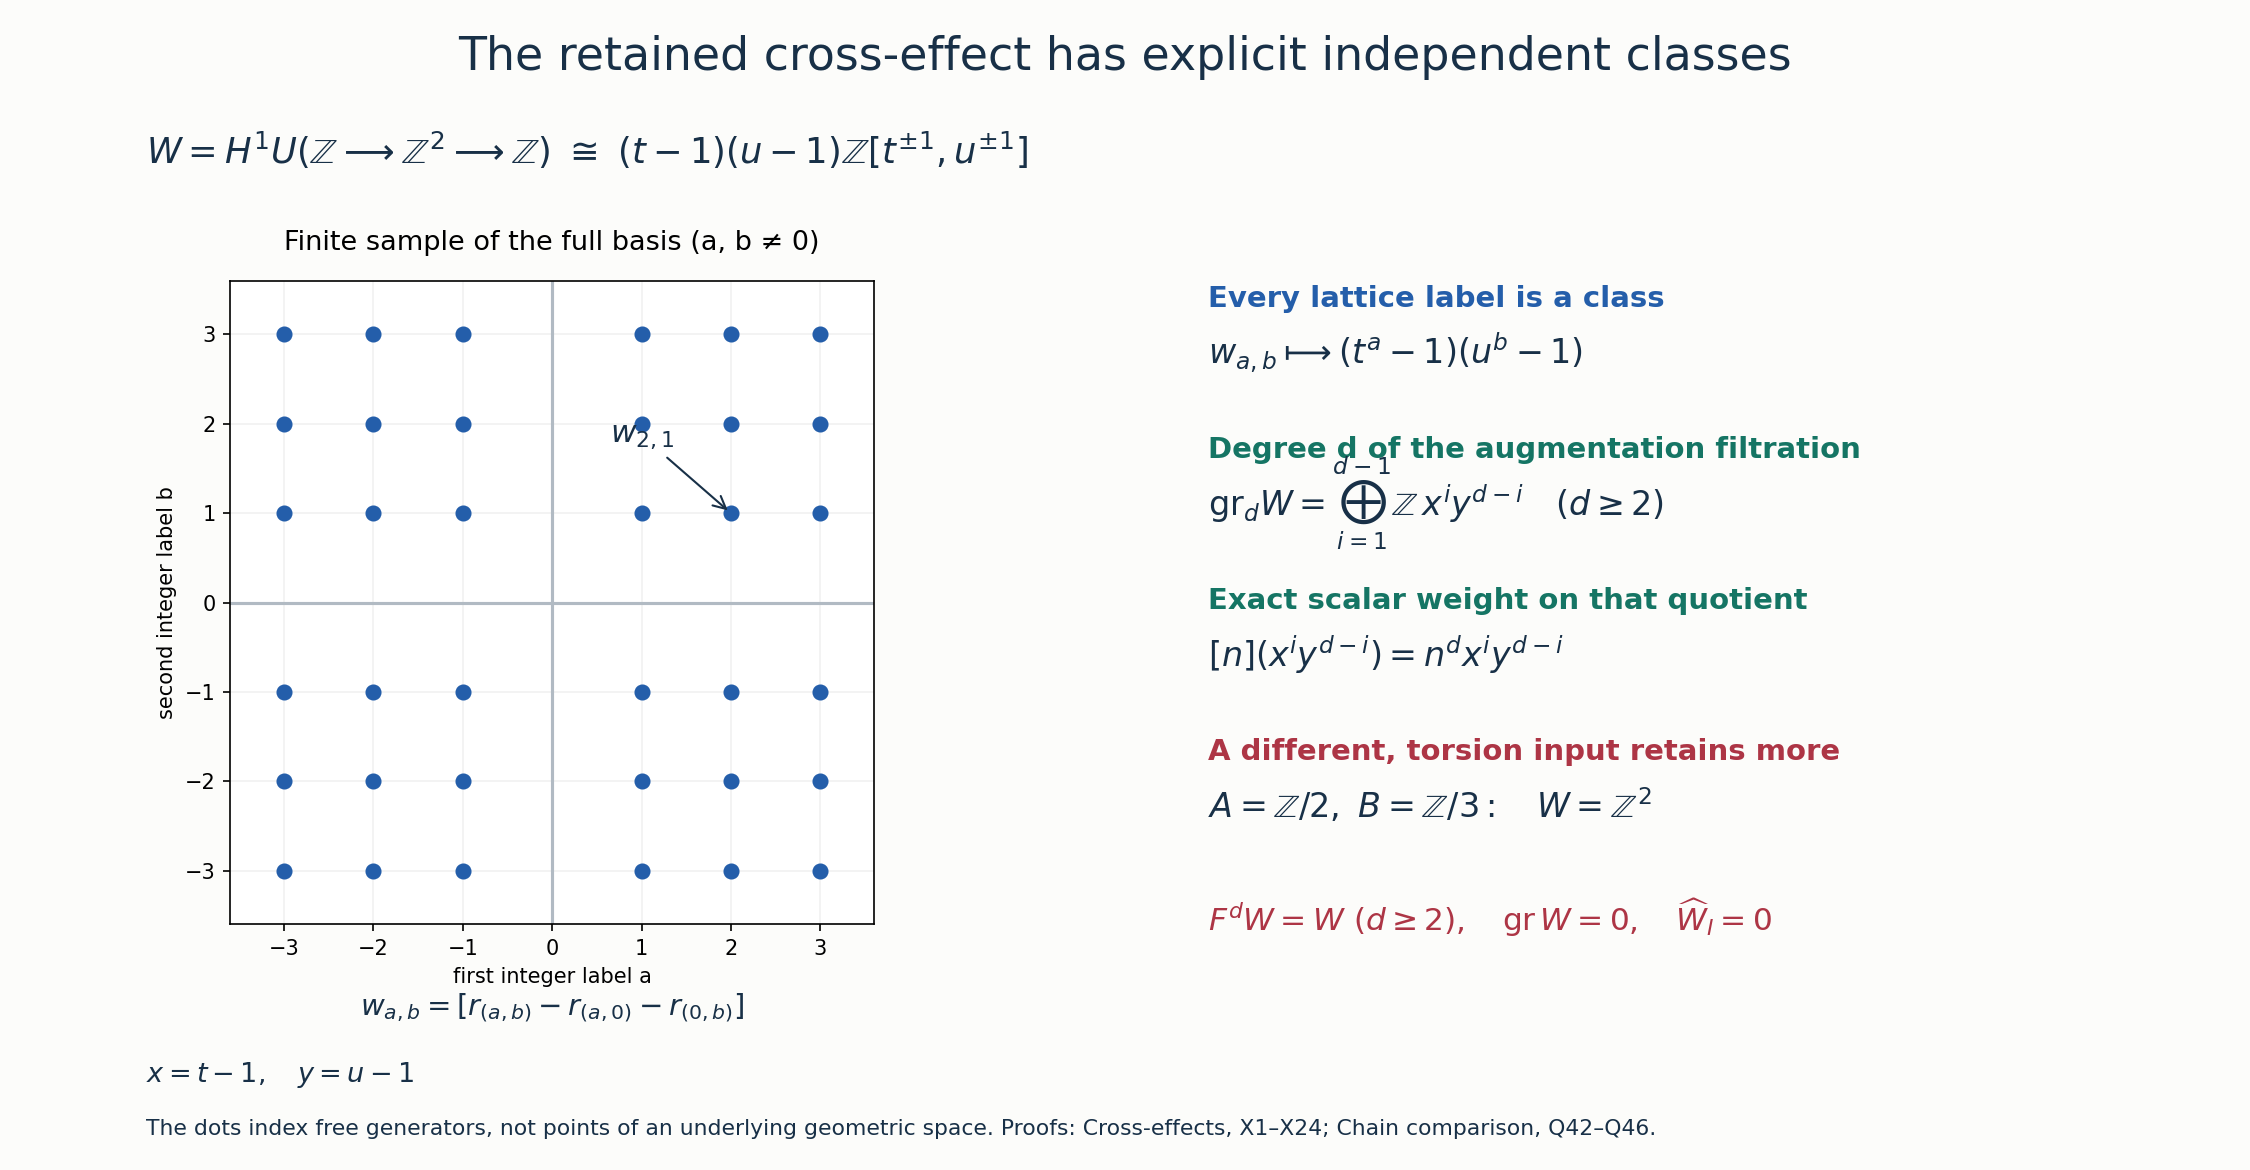
\includegraphics[keepaspectratio,alt={The retained classes and their filtration}]{figures/11_retained_cross_effect.png}}
\caption{The retained classes and their filtration}
\end{figure}

The grid is a finite sample of the independent basis (X3) for the
integer pair; the full basis includes all nonzero signed pairs. The
augmentation coordinates in the right panel are \(x=t-1,y=u-1\).
Equations (X19)--(X22) give the exact filtration and the different
torsion example. The source for the standard cross-effect definition is
uit de Bos--Taelman, Section 2, cited above; all concrete calculations
and maps used here are fully proved in this paper.

\end{document}
